\documentclass[conference]{IEEEtran}
\IEEEoverridecommandlockouts
% The preceding line is only needed to identify funding in the first footnote. If that is unneeded, please comment it out.
\usepackage{amsmath,amssymb,amsfonts}
\usepackage{algorithmic}
\usepackage{graphicx}
\usepackage{textcomp}
\usepackage{xcolor}
\usepackage[sort, numbers]{natbib}
\def\BibTeX{{\rm B\kern-.05em{\sc i\kern-.025em b}\kern-.08em
    T\kern-.1667em\lower.7ex\hbox{E}\kern-.125emX}}

% Make font size smaller in bibliography, as per:
% https://tex.stackexchange.com/questions/386709/proper-usage-of-biblatex-ieee-biblatex-style-in-an-ieeetran-document
\renewcommand*{\bibfont}{\footnotesize}

% begin pandoc tex stuff

\usepackage{hyperref}


\providecommand{\tightlist}{%
  \setlength{\itemsep}{0pt}\setlength{\parskip}{0pt}}

% end pandoc tex stuff

\begin{document}

\title{Joker: A Unified Interaction Model For Web Customization}

% removing authors for anonymous submission

% \author{\IEEEauthorblockN{1\textsuperscript{st} Given Name Surname}
% \IEEEauthorblockA{\textit{dept. name of organization (of Aff.)} \\
% \textit{name of organization (of Aff.)}\\
% City, Country \\
% email address or ORCID}
% \and
% \IEEEauthorblockN{2\textsuperscript{nd} Given Name Surname}
% \IEEEauthorblockA{\textit{dept. name of organization (of Aff.)} \\
% \textit{name of organization (of Aff.)}\\
% City, Country \\
% email address or ORCID}
% \and
% \IEEEauthorblockN{3\textsuperscript{rd} Given Name Surname}
% \IEEEauthorblockA{\textit{dept. name of organization (of Aff.)} \\
% \textit{name of organization (of Aff.)}\\
% City, Country \\
% email address or ORCID}
% \and
% \IEEEauthorblockN{4\textsuperscript{th} Given Name Surname}
% \IEEEauthorblockA{\textit{dept. name of organization (of Aff.)} \\
% \textit{name of organization (of Aff.)}\\
% City, Country \\
% email address or ORCID}}

\maketitle

\begin{abstract}
Tools that enable end-users to customize websites typically use a
two-stage workflow: first, users extract data into a structured form;
second, they use that extracted data to augment the original website in
some way. This two-stage workflow poses a usability barrier because it
requires users to make upfront decisions about what data to extract,
rather than allowing them to incrementally extract data as they augment
it.

In this paper, we present a new, unified interaction model for web
customization that encompasses both extraction and augmentation. The key
idea is to provide users with a spreadsheet-like formula language that
can be used for both data extraction and augmentation. We also provide a
programming-by-demonstration (PBD) interface that allows users to create
data extraction formulas by clicking on elements in the website. This
model allows users to naturally and iteratively move between extraction
and augmentation.

To illustrate our unified interaction model, we have implemented a tool
called Joker which is an extension of Wildcard, a prior web
customization system. Through case studies, we show that Joker can be
used to customize many real-world websites. We also present a formative
user study with five participants, which showed that people with a wide
range of technical backgrounds can use Joker to customize websites, and
also revealed some interesting limitations of our approach. Finally, we
present a heuristic evaluation of our design using the Cognitive
Dimensions framework.
\end{abstract}

\begin{IEEEkeywords}
end-user web customization, programming-by-demonstration, spreadsheets, end-user web scraping, program synthesis
\end{IEEEkeywords}

\hypertarget{sec:introduction}{%
\section{Introduction}\label{sec:introduction}}

Many websites do not meet the exact needs of all of their users, so
millions of people use browser extensions and userscripts
\citep{zotero-224, 2021f} to customize them. However, these tools only
allow end-users to install customizations built by programmers. End-user
web customization systems like Sifter \citep{huynh2006}, Vegemite
\citep{lin2009} and Wildcard \citep{litt2020} provide a more accessible
approach, allowing anyone to create bespoke customizations without
performing traditional programming.

These tools each provide different useful mechanisms for end-user
customization, but they share a common design limitation: they have a
rigid separation between the two stages of the web customization
process. First, in the \emph{extraction} or \emph{scraping} phase, users
get data from the website into a structured, tabular format. Second, in
the \emph{augmentation} phase, users perform augmentations like adding
new columns derived from the data, or sorting the data. For example, in
Vegemite, a user can extract a list of addresses from a housing catalog,
and then augment the data by computing a walkability score for each
address.

This separation between extraction and augmentation poses an important
barrier to usability. A user study \citep{lin2009} of Vegemite wrote
that ``it was confusing to use one technique to create the initial
table, and another technique to add information to a new column.'' The
creators of Sifter similarly reported \citep{huynh2006} that ``the
necessity for extracting data before augmentation could take place was
poorly understood, if understood at all.'' In Wildcard, end-users cannot
augment a website at all until a programmer has written and shared
extraction code for that website in Javascript \citep{litt2020}. These
tools all impose a sequential workflow in which users must first extract
all the data they need, and then perform all their desired
augmentations. This workflow exemplifies the more general problem in
interface design of forcing users to make premature commitments to
formal structure \citep{shipman1999, blackwell2001}.

In this paper, we present a new approach to web customization that
combines extraction and augmentation in a unified interaction model. Our
key idea is to develop a domain specific language (DSL) that encompasses
both extraction and augmentation tasks, along with a
programming-by-demonstration (PBD) interface that makes it easy for
end-users to program in the language. This unified interaction model
allows end-users to move seamlessly between extraction and augmentation,
resulting in a more iterative and free-form workflow for web
customization.

To demonstrate and evaluate this model, we have built a browser
extension called Joker, an extension of the Wildcard customization tool.
The original Wildcard system \citep{litt2020} adds a spreadsheet-like
table to a website and establishes a bidirectional synchronization
between the website and the table. This allows users to customize a
website, by filtering and sorting page elements, and adding user
annotations, derived values and calls to web services. Although Wildcard
offers a declarative formula language for augmenting the page, a
conventional imperative language (namely JavaScript) is used for the
extraction step, and the extraction code cannot be modified during
augmentation.

Joker makes two primary contributions:

\textbf{A unified formula language for extraction \& augmentation}:
Wildcard's formula language only supported primitive values like strings
and numbers aimed at augmentation. Joker extends this language by
introducing Document Object Model (DOM) elements as a new type of value,
and adding a new set of formulas for performing operations on them. This
includes querying elements with Cascading Style Sheets (CSS) selectors
and traversing the DOM. With this approach, a single formula language is
used to express both extraction and augmentation tasks, even within a
single formula expression.

\textbf{A PBD interface for creating extraction formulas}: Directly
writing extraction formulas can be challenging for end-users, so Joker
provides a PBD interface that synthesizes formulas from user
demonstrations. A key aspect of our design is that the program
synthesized from the demonstration is made visible as a spreadsheet
formula that can be subsequently edited by the user, and is more easily
understood than imperative code due to its declarative form.

Section~\ref{sec:examples} describes a concrete scenario, showing how
Joker enables a user to complete a useful customization task. In
Section~\ref{sec:implementation}, we outline the implementation of our
formula language and user interface, as well as the algorithms used by
our PBD interface.

We have performed three evaluations of our approach, presented in
Section~\ref{sec:evaluation}. First, we describe a suite of case studies
in which we used Joker to extract and augment a variety of websites in
order to characterize its capabilities and limitations. Second, we
describe a formative user study with five participants, which showed
that users were generally able to use Joker to perform useful extraction
and augmentation tasks, but which also uncovered limitations,
particularly for less experienced users trying to extract data from more
complex websites. Finally, we perform a heuristic evaluation of our
design, using the Cognitive Dimensions \citep{blackwell2001} framework.

Joker relates to existing work not only in end-user web customization,
but also in end-user web scraping and program synthesis, which we
discuss in Section~\ref{sec:related-work}. Finally, we discuss
opportunities for future work in Section~\ref{sec:conclusion}.

\hypertarget{sec:examples}{%
\section{Example Usage Scenario}\label{sec:examples}}

Here is an example scenario, illustrated in Figure~\ref{fig:ebay}, and
demonstrated in the video accompanying this paper. Jen is searching for
a karaoke machine on eBay, a shopping website. She wants to use Joker to
sort products by price within a page of search results, a feature not
supported by eBay.

\begin{figure*}
  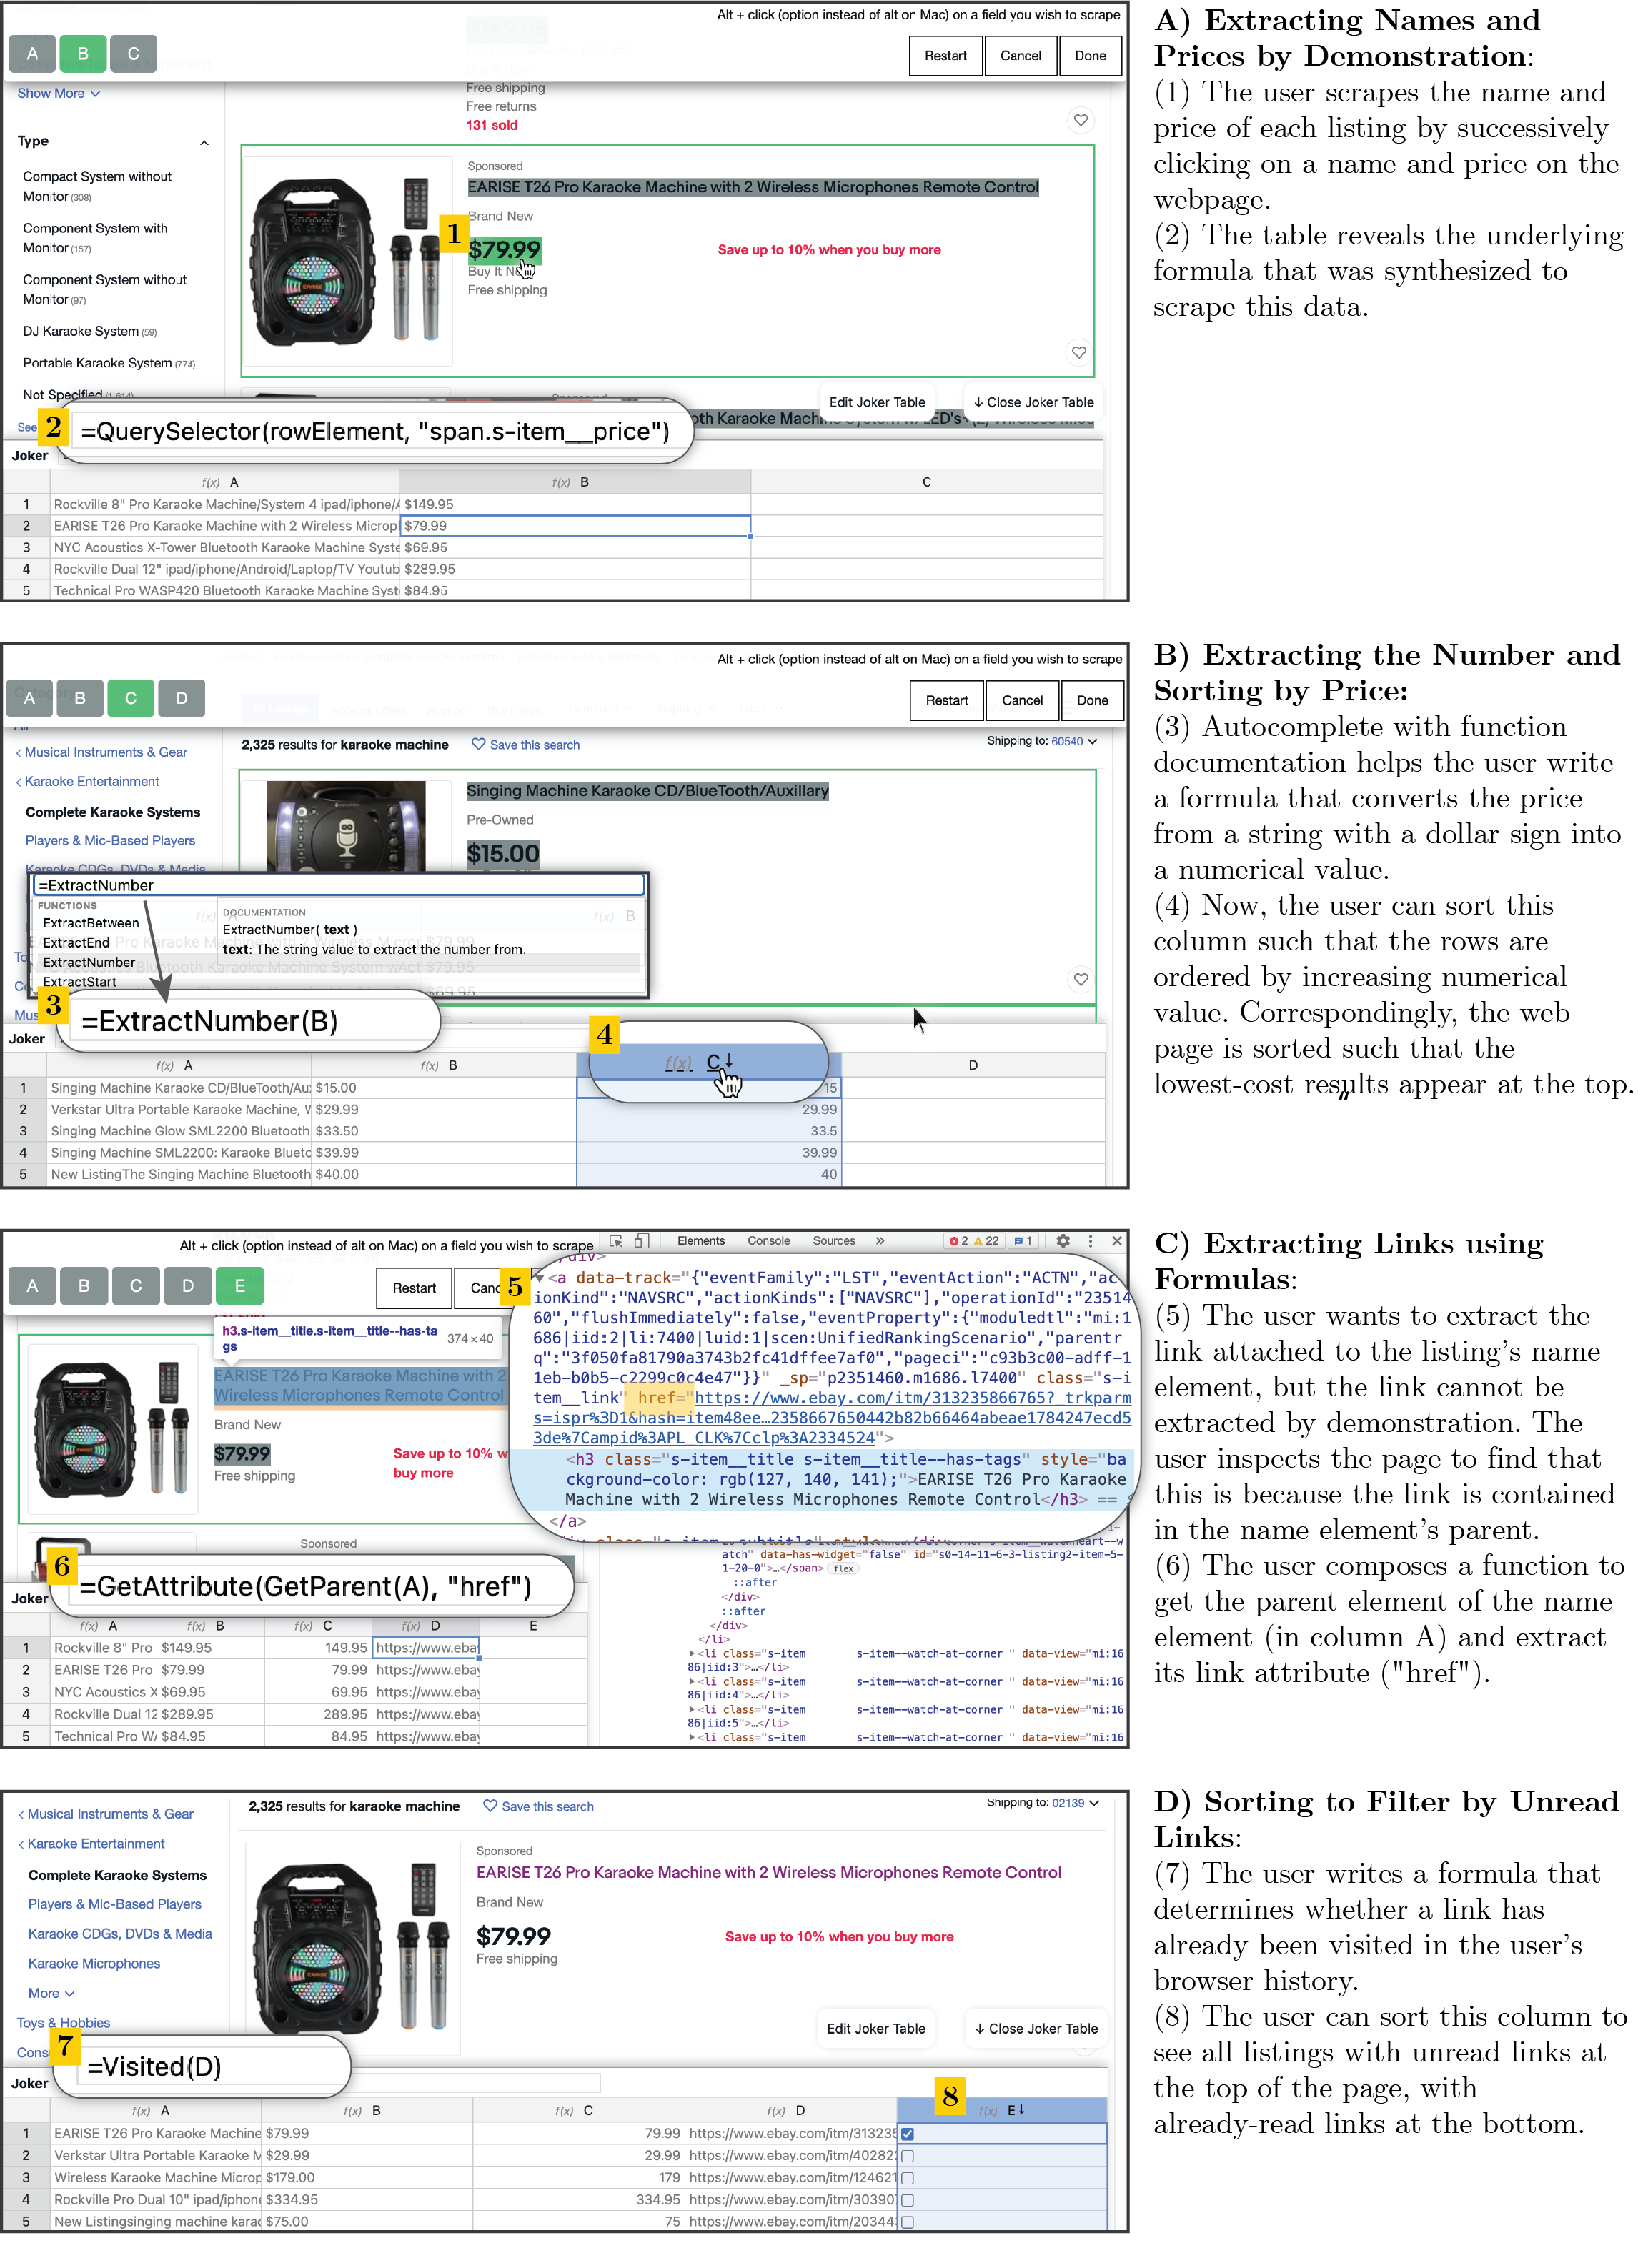
\includegraphics[width=\textwidth]{media/ebay.png}
  \caption{\label{fig:ebay}Scraping and customizing eBay by unified demonstration and formulas.}
\end{figure*}

\emph{Extracting Product Titles \& Prices By Demonstration}.
(Figure~\ref{fig:ebay} Part A): Jen initiates Joker through the browser
context menu. As she hovers over the product title, Joker provides two
kinds of live feedback. First, it highlights the titles of all the
corresponding product listings on the page, to indicate how it has
generalized Jen's intent based on her demonstration of a single example
product. Second, a column of the table is populated with the values that
will be extracted, giving a preview of how the extracted data would
look. To commit to this extraction, Jen clicks on the product title. She
repeats a similar process to extract the price.

When she clicks one of the cells in column \texttt{B}, the formula bar
above the table displays the extraction formula that was generated from
her demonstration:

\texttt{=QuerySelector(rowElement,\ "span.s-item\_\_price")}

This formula produces the values in column \texttt{B}. For each row in
the table, Joker has a created a reference to the corresponding DOM
element, accessible through the special identifier \texttt{rowElement}.
The \texttt{QuerySelector} function runs the specified CSS selector
(\texttt{span.s-item\_\_price}) within the row element to extract the
price of each item. While Jen could directly edit this formula, in this
case the values in the table are correct, so there's no need to edit the
formula.

\emph{Sorting Products By Price}. (Figure~\ref{fig:ebay} Part B): Next,
Jen wants to sort the table by price, but she realizes that the column
of prices is a list of strings containing the \texttt{\$} symbol. She
needs to \emph{augment} this raw data by turning the strings into
numbers. In the next column (\texttt{C}), Jen starts typing a formula,
and uses an autocomplete dropdown to find a relevant function that
extracts numeric values from strings:

\texttt{=ExtractNumber(B)}

Now column C contains numeric values, so Jen can sort the table by
price. Because the table is synchronized with the website, the product
listings become sorted as well.

\emph{Extracting Product URL With Formulas} (Figure~\ref{fig:ebay} Part
C): While completing the previous task, Jen realizes there is another
customization she would find useful: prioritizing products for which she
has not yet visited the details page for the listing. To do this, she
must first return to \emph{extracting} more relevant data from the page.

Each product listing links to a page for the specific product, but
because the URL is not visible in the page, it's not possible to
directly extract it by demonstration. However, Jen can still achieve the
goal by directly writing an extraction formula.

Jen has some basic knowledge of HTML, which she can leverage to write
the formula. She opens the browser developer tools, and observes that
the listing title is represented by a link tag with a heading inside:

\begin{verbatim}
<a href="LISTING PAGE URL">
  <h3>LISTING NAME</h3>
</a>
\end{verbatim}

Since there is already a column \texttt{A} in the table representing the
product's title, she can use this as a starting point to write the
formula:

\texttt{=GetAttribute(GetParent(A),\ "href")}

This formula first calls the \texttt{GetParent} function on column
\texttt{A}, traversing up a level from the
\texttt{\textless{}h3\textgreater{}} elements to the
\texttt{\textless{}a\textgreater{}} elements. Then,
\texttt{GetAttribute} extracts the \texttt{href} value containing the
link URL. After running this formula, the table contains a column
\texttt{D} with the URL for each product.

\emph{Sorting Products By Whether They Have Been Visited}
(Figure~\ref{fig:ebay} Part C): After performing that extraction, Jen
can write a final augmentation formula to indicate whether she has
visited the corresponding product page:

\texttt{=Visited(D)}

The \texttt{Visited} function checks whether a URL is present in the
browser history and returns a boolean value represented by a checkbox.
Jen can then sort by this column to put listings that she has not yet
visited at the top of the page.

Using Joker, Jen was able to not only achieve her initial customization
goal to sort the products by price but also perform a customization she
did not plan to do. This was made possible by Joker's unified
interaction model for web customization which enabled her to interleave
extraction and augmentation. While we have described only a single
illustrative scenario in this example, Joker is flexible enough to
support a wide range of other useful customizations and workflows on
various websites, described in more detail in
Section~\ref{sec:evaluation}.

\hypertarget{sec:implementation}{%
\section{System Implementation}\label{sec:implementation}}

\begin{figure*}
  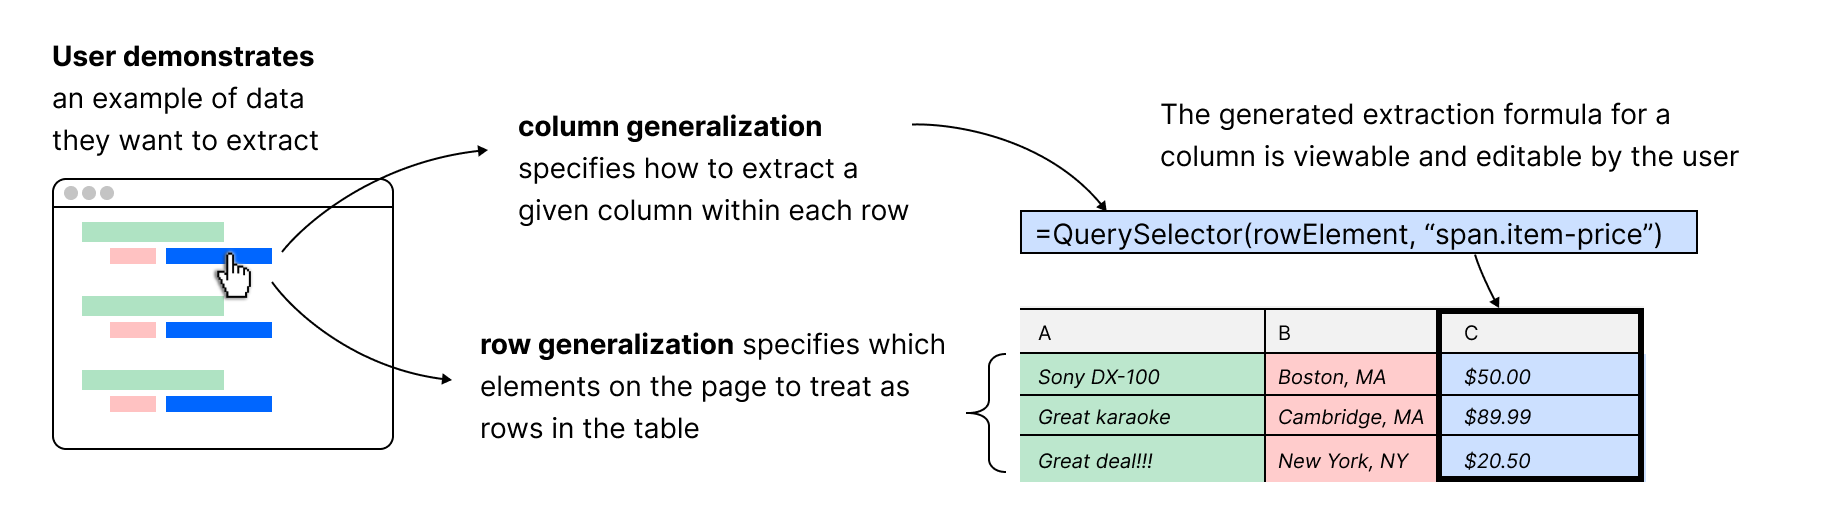
\includegraphics[width=\textwidth]{media/overview.png}
  \caption{\label{fig:overview}An overview of Joker's interaction model and wrapper induction process.}
\end{figure*}

In this section, we describe Joker's formula language in more detail.
Then, we outline the \emph{wrapper induction} \citep{kushmerick2000}
algorithm that Joker's PBD interface uses to synthesize the row element
and column selectors presented in formulas. Figure~\ref{fig:overview}
illustrates the entire process.

\hypertarget{extraction-formulas}{%
\subsection{Extraction Formulas}\label{extraction-formulas}}

The Wildcard customization tool includes a formula language for
augmentation, including operators for basic arithmetic and string
manipulation, as well as more advanced operators that fetch data from
web APIs. As in other tabular interfaces like SIEUFERD \citep{bakke2016}
and Airtable \citep{2021f}, formulas apply to a whole column at a time
rather than a single cell, and can reference other columns by name.
Joker extends this base language with new constructs which enable it to
apply to \emph{data extraction} instead of just augmentation.

We added DOM elements as a data type in the language, alongside strings,
numbers, and booleans. Because the language runs in a JavaScript
interpreter, we simply use native JavaScript values to represent DOM
elements in the language. DOM elements are displayed visually by showing
their inner text contents. They can also be implicitly typecast to
strings for use in other formulas; for example, a string manipulation
formula like \texttt{Substring} can be called on a DOM element value,
and will operate on its text contents.

We also added several functions to the formula language for traversing
the DOM and performing extractions, summarized below with their types:

\begin{itemize}
\tightlist
\item
  \texttt{QuerySelector(el:\ Element,\ sel:\ string):\ Element}.
  Executes the CSS selector \texttt{sel} inside of element \texttt{el},
  and returns the first matching element.
\item
  \texttt{GetAttribute(el:\ Element,\ attribute:\ string):\ string}.
  Returns the value for an attribute on an element.
\item
  \texttt{GetParent(el:\ Element):\ Element}. Returns the parent of a
  given element.
\end{itemize}

To extract data from a row, formulas need a way to reference the current
row, so we added a construct to support this use case. Every row in the
table maps to one DOM element in the page; we allow formulas to access
this DOM element via a special keyword, \texttt{rowElement}. In some
sense, \texttt{rowElement} can be seen as a hidden extra column of data
in the table containing DOM elements.

While many more functions could be added to expose more of the
underlying DOM API, we found that in practice these three functions
provided ample power through composition. For example, in
Section~\ref{sec:examples} we showed how \texttt{GetParent} and
\texttt{GetAttribute} can be composed to traverse the DOM and extract
the URL associated with a product listing.

By providing a single formula language to express extractions and
augmentations, Joker enables a \emph{unified interaction model} that
supports interleaving the two. Furthermore, the formula language enables
users to specify logic using pure, stateless functions that reactively
update in response to upstream changes. This \emph{functional reactive
paradigm} is easier to reason about than traditional imperative
programming, as demonstrated by the use of formulas by millions of end
users in spreadsheet programs and end-user programming environments
\citep{2021g, 2021h, 2021f, 2021a, 2021c, chang2014}.

\hypertarget{wrapper-induction}{%
\subsection{Wrapper Induction}\label{wrapper-induction}}

When users demonstrate a specific column value to extract, Joker must
synthesize a program that reflects the user's general intent. This is an
instance of the \emph{wrapper induction} problem of synthesizing a web
data extraction query from examples. Prior work on this topic
\citep{kushmerick2000, furche2016} prioritizes accuracy and robustness
to future changes, which makes sense for a fully automated system, but
can lead to very complex queries. In our work, we chose to prioritize
the readability of queries by less sophisticated users, so that users
can more easily author queries and repair them when they break. We
implemented a set of heuristics inspired by Vegemite \citep{lin2009} for
wrapper induction, described below.

\hypertarget{determining-row-elements}{%
\subsubsection{Determining Row
Elements}\label{determining-row-elements}}

The user starts by demonstrating an element \(v\), representing a value
that should be in the table. From that demonstration, we must find a set
of \emph{row elements} that represent the rows of the table. We could
naively assume that \(parent(v)\) is the row containing \(v\), but often
\(v\) is deeply nested inside its containing row; we must determine
which ancestor of \(v\) is likely to be the row.

Intuitively, we solve this problem by assuming that all rows share some
similar internal structure. In particular, we expect most rows to
contain a value for the demonstrated column. (If there were no missing
data, we'd expect \emph{all} rows to contain data for this column.)

Formally: assume a function \(select(el, s)\) which runs a CSS selector
that returns the set of elements matching \(s\) within \(el\). We
generate a set of plausible candidates \(P\), consisting of pairs of a
row element and a CSS selector:

\(P = \{ (r, s) \mid r \in ancestors(v) \land select(r, s) = \{v\} \}\)

For each candidate \((r, s) \in P\), we compute a weight function \(w\),
which is based on the number of siblings of \(r\) that have ``similar
structure'', defined by checking whether running \(s\) within the
sibling also returns a unique element.

\(w(r, s) = |\{ r' \mid r' \in siblings(r) \land |select(r', s) | = 1 \}|\)

We then choose the candidate with the highest weight. In case of ties,
the candidate closer to \(v\) in the tree (i.e., lower in the tree)
wins. Given a winning candidate \((r, s)\), the full set of row elements
is \(\{r\} \cup siblings(r)\).

\hypertarget{synthesizing-css-selectors-for-column-values}{%
\subsubsection{Synthesizing CSS Selectors For Column
Values}\label{synthesizing-css-selectors-for-column-values}}

Once we have determined the row elements, next we must choose a CSS
selector that will be used to identify the demonstrated value within its
row.

Given a demonstrated value \(v\) within a row element \(r\), we generate
two kinds of plausible selectors:

\begin{itemize}
\tightlist
\item
  selectors using CSS classes, which are manual annotations on DOM
  elements added by the website's programmers, typically for styling
  purposes (e.g.~"item\_\_price")
\item
  selectors using positional indexes within the tree, using the
  \texttt{nth-child} CSS selector (e.g.~\texttt{nth-child(2)},
  representing the second child of an element)
\end{itemize}

The minimum criteria for a plausible selector \(s\) is that it uniquely
identifies the value within the row: \(select(r, s) = \{v\}\). But there
may be many plausible selectors, so we must pick a best one.

We first prioritize selectors using classes, because they tend to be
more robust to changes on the website. A single selector can combine
multiple classes, but we prefer using fewer classes when possible. If no
plausible class-based selector can be generated (for example, if the
relevant elements don't have any classes to query), we fall back to
using a positional index selector. This kind of selector can always be
generated regardless of the contents of the page, but tends to be less
accurate and robust.

\hypertarget{sec:evaluation}{%
\section{Evaluation}\label{sec:evaluation}}

We evaluate our interaction model and tool in terms of three research
questions:

\emph{RQ1: What kinds of websites can this model operate effectively
on?} We evaluate this with a suite of case studies that demonstrate its
capabilities and limitations.

\emph{RQ2: How are users of different backgrounds able to use the
system?} We evaluate this with a small formative user study.

\emph{RQ3: What are the essential design dimensions that distinguish
this model from other approaches?} We evaluate this with a heuristic
analysis using the Cognitive Dimensions of Notation framework
\citep{blackwell2001}.

\hypertarget{case-studies}{%
\subsection{Case Studies}\label{case-studies}}

Our first evaluation describes the results of the authors using Joker to
extract data and perform customizations on popular websites. For the
websites on which Joker can be used, we provide the sequence of
interactions needed to achieve the customizations; for the websites on
which Joker fails, we explain the relevant limitations.

\hypertarget{successful-applications}{%
\subsubsection{Successful Applications}\label{successful-applications}}

\begin{table*}[]
\centering
\begin{tabular}{|l|l|}
\hline
\textbf{Website}              & \textbf{Example Customization Achieved by Joker}                                        \\ \hline
eBay, Amazon            & Filter listings by whether they have a "Sponsored" label.                        \\
Amazon, Target & Sort search results by price and rating.                                                \\
Google Scholar                & Filter publications for those whose title contains a user-provided keyword. \\
Reddit, CNN, ABC  & Sort by the read times of articles. Filter already-visited articles.         \\
Weather.com                   & Filter hourly weather to find sunny times of day.                                        \\
Github                        & Sort a user's code repositories by stars to find popular work.                          \\
Postmates, Uber Eats    & Sort restaurants by delivery time and delivery fee.                                     \\ \hline
\end{tabular}
\vspace{8pt}
\caption{Examples of websites that Joker can be used to customize, including extraction and augmentation}
\end{table*}

We have used Joker to achieve a variety of customizations across many
websites. Table 1 summarizes examples we have found on popular websites.

\emph{Sorting search results by price on Amazon.} We have found Joker to
be useful for sorting the contents of various websites. One example of a
useful sort achieved by Joker is sorting search results by price within
the Featured page on Amazon. (Using Amazon's sort by price feature often
returns irrelevant results.) In Amazon's source code, the price is split
into three HTML elements: the dollar sign, the dollar amount, and the
cents amount. A user can extract by demonstration only the cents element
into column \texttt{A}. Subsequently, because the parent element of the
cents element contains all three of the price elements, the user can
extract the full price using the formula \texttt{GetParent(A)}. Next,
the user can write the formula \texttt{ExtractNumber(B)} to convert the
string into a numeric value. Finally, the user can sort this column by
low-to-high prices. In a similar manner, we have used Joker to extract
and sort prices and ratings on the product listing pages of Target and
eBay.

\emph{Filtering titles of publications on Google Scholar.} We have also
found Joker can be useful for filtering a website's listings based on
the text content of an element in the listing. For example, we have used
Joker to filter the titles of a researcher's publications on their
Google Scholar profile which is not natively supported. First, a user
can extract the titles into a column (\texttt{A}) by demonstration.
Then, the user can write the formula \texttt{Includes(A,\ "compiler")}
that returns whether or not the title contains the keyword ``compiler''.
Finally, the user can sort by this column to get all of the publications
that fit their constraint at the top of the page. We have also used
Joker to filter other text-based directory web pages such as Google
search results and the MIT course catalog, in similar ways.

\emph{Retrieving information about links on Reddit.} Additionally, we
have used Joker to augment web pages with external information. For
example, Joker can augment Reddit's user interface, which has a list of
headlines with links to articles, with the links' read times and whether
the link has already been read. To achieve this customization, a user
first extracts the headline elements into column (\texttt{A}) by
demonstration. The user can then extract the link into the next column
(\texttt{B}) with the formula \texttt{GetAttribute(A,\ "href")}. Then,
the user can write the formula \texttt{ReadTimeInSeconds(B)} that calls
an API that returns the links' read times. Similarly, the user can write
the formula \texttt{Visited(B)}, which uses another API that returns
whether that link has been visited in the user's browser history. The
user can also extract elements such as the number of comments and the
time of posting and sort by these values. We have performed similar
customizations on websites such as ABC News and CNN.

\hypertarget{limitations}{%
\subsubsection{Limitations}\label{limitations}}

Joker is most effective on websites whose data is presented as a
collection of similarly-structured HTML elements. Certain websites,
however, have designs that make it difficult for Joker to extract data:

\begin{itemize}
\tightlist
\item
  \emph{Heterogeneous row elements.} Some websites break their content
  into rows, but the rows do not have a consistent layout, and contain
  different types of child elements. For example, the page design of
  HackerNews alternates between rows containing a title and rows
  containing supplementary data (e.g.~number of likes and the time of
  posting). Because Joker only chooses a single row selector, when
  extracting by demonstration, Joker will only select one of the types
  of rows, and elements in the other types of rows will not be
  extracted.
\item
  \emph{Infinite scroll.} Some websites have an ``infinite scroll''
  feature that adds new entries to the page when a user scrolls to the
  bottom. Joker's table will only contain elements that were rendered
  when the table was first created. Additionally, for websites that
  render a very large number of DOM elements, the speed of the live
  feedback provided by Joker's PBD interface might significantly
  decrease. This is because the wrapper induction process used by the
  PBD interface queries the DOM which takes longer as the size of the
  DOM increases.
\end{itemize}

\hypertarget{user-study}{%
\subsection{User Study}\label{user-study}}

We conducted a small formative user study to understand how people would
interact with Joker.

\hypertarget{participants}{%
\subsubsection{Participants}\label{participants}}

We recruited 5 participants with varying backgrounds. 3 participants
were familiar with spreadsheet formulas. 3 participants had extensive
web development experience, 1 had a small amount of prior web
development experience, and 1 had no web development experience. 3
participants had previously extracted data from websites.

\hypertarget{protocol}{%
\subsubsection{Protocol}\label{protocol}}

The participants completed 7 web customization tasks across 2 websites.
All participants attempted all the tasks.

First, we asked participants to customize a website with a relatively
simple HTML structure: the MIT EECS course catalog website. All data
\emph{extraction} on this site can be performed with demonstrations
alone in Joker, although augmentation still requires writing formulas.
The specific tasks were the following: 1a) Extract course titles, 1b)
Extract course prerequisites, 1c) Add a column that indicates whether a
course has a prerequisite \& 1d) Add a column that indicates whether a
course has no prerequisites and is offered in the fall term.

Next, we asked participants to customize a website with a more complex
HTML structure: the search results page for the eBay shopping website.
Due to the website's complexity, demonstrations alone are not sufficient
to extract data; users must also directly edit extraction formulas. The
specific tasks were the following: 2a) Extract title from listings of
Apple iPhones for sale, 2b) Extract the listing price for the phone, \&
2c) Create a column that indicates whether a listing for a phone is
sponsored.

Each session was 60 minutes long and conducted over a recorded video
conference. We started each session with a description of Joker and
provided a brief tutorial of its main features on a sample website not
used in the tasks. There was no time limit for completing the tasks.
Users were encouraged to speak aloud as they worked.

Because some of the tasks build on results of previous tasks, we wanted
to ensure all participants made enough progress to gather useful
feedback. Therefore, whenever a participant got stuck for several
minutes, we recorded why they were stuck and then offered hints on how
to proceed (such as suggestions to read formula documentation or open
the browser dev tools). While all participants were able to complete all
tasks with hints, this obviously does not mean they could have completed
the task unassisted. Our goal was not to simply measure whether users
completed the task, but rather to gain qualitative insight into the
barriers they faced.

\hypertarget{results}{%
\subsubsection{Results}\label{results}}

\emph{Unified interaction model.} Most participants took advantage of
the unified interaction model to interleave extraction and augmentation
tasks, rather than performing all extraction up front. For example, on
task 1, most participants extracted the prerequisites by demonstration,
added one or more columns to the table to perform some string operations
on the prerequisites, and then continued on to extract more information
from the web page by demonstration. Furthermore, we hypothesize that in
a less controlled setting, users would be even more likely to interleave
extraction and augmentation, since the task may be less well defined at
the beginning.

One usability issue with the unified model was that participants
sometimes got confused about how their demonstrations would affect the
contents of the table. For example, multiple participants intended to
add a new column by demonstrating an extraction, but instead
accidentally overwrote the contents of an existing column. This poses a
design challenge because the user's demonstrations occur in the website,
so they cannot directly interact with the table while demonstrating;
this suggests that the interface needs to do a better job indicating
where the results of a demonstration will be inserted.

\emph{Extracting simple data.} On the relatively simple MIT course
catalog website, all participants were able to extract the relevant data
from the page within seconds, simply performing demonstrations with a
few clicks. This suggests that when Joker's generalization algorithm
works well, it can be an effective tool for data extraction, even for
users with limited programming experience. P1 said: \emph{``you could
hover and {[}the data{]} was already selected\ldots that was very
nice''}. P3, upon seeing the tutorial for extraction by demonstration,
said \emph{``that's like black magic.''}

\emph{Extracting complex data.} On the more complex eBay website where
demonstration alone was not sufficient, results were more varied. P1,
who had no prior web development experience, struggled to complete the
task, saying that \emph{``looking at HTML is a bit much''}; this
suggests that more work could be done to make the experience usable for
novices. However, users with more web development experience were able
to use the tool to perform complex extractions, such as directly writing
CSS selectors into the formula bar. P2 and P3 both reported that Joker's
live feedback loop was easier to use and faster than other approaches to
web extraction; P3 noted that \emph{``{[}with any other approach{]}, it
would have been slower to specify and slower to validate that I
specified it correctly.''}

It was challenging for some participants to switch between using the
browser's developer tools and the Joker interface when doing complex
extraction tasks. While we chose not to build HTML inspection into the
Joker UI because the browser already provides a very rich set of tools,
users sometimes were not able to tell how elements in the Joker table
corresponded to elements in the browser's element inspector.

\emph{Writing formulas.} In general, participants were able to learn the
formula language by using an autocomplete dropdown with inline
documentation, which we developed as part of the Joker extension. In
some cases, participants were able to immediately construct correct
formulas on the first try; in other cases it took several attempts and
some hints from the moderator to try a relevant function. While better
documentation and error messages could help improve the learnability of
the formula language, we also did not find it surprising that
participants required some time to learn a completely unfamiliar formula
language.

\hypertarget{cognitive-dimensions-analysis}{%
\subsection{Cognitive Dimensions
Analysis}\label{cognitive-dimensions-analysis}}

We analyzed Joker using the Cognitive Dimensions of Notation
\citep{blackwell2001}, a heuristic evaluation framework that has been
used to evaluate programming languages and visual programming systems
\citep{satyanarayan2014, satyanarayan2014a, ledo2018}. When contrasting
our tool with other scraping and customization tools, we find
particularly meaningful differences along several dimensions:

\emph{Progressive evaluation.} In Joker, a user can see the intermediate
results of their extraction and augmentation work at any point, and
adjust their future actions accordingly. The table user interface makes
it easy to inspect the intermediate results and notice surprises like
missing values.

In contrast, traditional extraction typically requires editing the code,
manually re-running it, and inspecting the results in an unstructured
textual format, making it harder to progressively evaluate the results.
Also, many end-user extraction tools \citep{chasins2018, lin2009}
require the user to demonstrate all the data extractions they want to
perform before showing any information about how those demonstrations
will generalize across multiple examples.\footnote{This is an instance
  where Joker's limitation of only scraping a single page at a time
  proves beneficial. All the relevant data is already available on the
  page without further network requests, making it possible to support
  progressive evaluation with low latency. Other tools that support
  scraping across multiple pages necessarily require a slower feedback
  loop.}

\emph{Premature commitment.} Many scraping tools require making a
\emph{premature commitment} to a data schema: first, the user extracts a
dataset, and then they perform augmentations using that data. Wildcard
suffered from this problem: when writing code for extraction, a user
would need to anticipate all future augmentations and extract the
necessary data.

Joker instead supports extracting data \emph{on demand}. The user can
decide on their desired augmentations and extract data as needed to
fulfill those tasks. There is never a need to eagerly guess what data
will be needed in advance.

We have also borrowed a technique from spreadsheets for avoiding
premature commitment: default naming. New data columns are automatically
assigned a single-letter name, so that the user does not need to
prematurely think of a name before extracting the data. We have not yet
implemented the capability to optionally rename demonstrated columns,
but it would be straightforward to do so, and would provide a way to
offer the benefits of names without requiring a premature commitment.

\emph{Provisionality.} Joker makes it easy to try out an extraction
action without fully committing to it. When the user hovers over any
element in a website, they see a preview of how that data would be
extracted into the table, and then they can click if they'd like to
proceed. This makes it feel very fast and lightweight to try scraping
different elements on the page.

\emph{Viscosity.} Some scraping tools have high viscosity: they make it
difficult to change a single part of an extraction specification without
modifying the global structure. For example, in Rousillon
\citep{chasins2018}, changing the desired demonstration for a single
column of a table requires re-demonstrating all of the columns. In
contrast, Joker allows a user to change the specification for a single
column of a table without modifying the others, resulting in a lower
viscosity in response to changes.

\hypertarget{sec:related-work}{%
\section{Related Work}\label{sec:related-work}}

Joker builds on existing work in end-user web customization, end-user
web scraping and program synthesis.

\hypertarget{end-user-web-customization}{%
\subsection{End-user Web
Customization}\label{end-user-web-customization}}

Joker builds on web customization ideas implemented by previous tools.
Our contribution is a new interaction model that allows for interleaving
extraction and augmentation, enabled by a unified formula language and a
PBD interface.

Joker is an extension of the Wildcard customization system
\citep{litt2020}, and preserves its foundational idea of synchronizing a
table with a website. Wildcard only allows for extraction logic to be
written by programmers in Javascript; our work has substantially
extended the Wildcard formula language and added an entire new system
for dynamically creating data extraction logic within the user
interface. We also improved the formula editing interface by adding an
autocomplete dropdown and documentation popup, which proved important in
our testing for allowing end-users to reliably edit and create formulas.

Vegemite \citep{lin2009} is a tool for end-user programming of web
mashups. Like Joker, it allows users to perform demonstrations to
extract data, but Vegemite only displays a table after all the
demonstrations have been provided, which rules out interleaving
extraction and augmentation. Vegemite does allow users to directly view
and edit some of the logic generalized from demonstrations, but it only
allows for editing augmentation logic, not extraction logic. The wrapper
induction algorithm used in Joker is also very similar to Vegemite's
algorithm.

Sifter \citep{huynh2006} is a tool that augments websites with advanced
sorting and filtering functionality. It attempts to automatically detect
items and fields on the website with a variety of heuristics. If these
fail, it gives the user the option of demonstrating to correct some
parts of the result. In contrast, Joker makes fewer assumptions about
the structure of websites, by giving control to the user from the
beginning of the process and displaying an editable synthesized program.
We hypothesize that focusing on a tight feedback loop rather than
automation may support a scraping process that offers more expressive
power and extends to a greater variety of websites, but further user
testing is required to validate this hypothesis. Of course, better
heuristics could benefit our model as well; the ideal system would make
good guesses while giving the user full understanding and control of the
extraction process.

\hypertarget{end-user-web-scraping-and-program-synthesis}{%
\subsection{End-user Web Scraping and Program
Synthesis}\label{end-user-web-scraping-and-program-synthesis}}

Joker builds on insights from other tools that synthesize web scraping
(i.e.~data extraction) code from user demonstrations, and give users
ways to inspect and modify the generated code.

Rousillon \citep{chasins2018} is a tool that enables end-users to
extract hierarchical web data across multiple linked web pages. It
presents the web extraction program generated from demonstrations in an
editable, high-level, block-based language called Helena \citep{2021c}.
While both Rousillon and Joker create an editable program, they have
different focuses. Because Rousillon allows users to extract data across
multiple pages (e.g., extracting details from each linked page in a
list), it uses an imperative language, with nested loops as a key
construct. In contrast, Joker can only extract within a single page, and
therefore can use a simpler declarative formula language. Also,
Rousillon only allows editing high-level control flow and treats some
details of the extraction logic as opaque; Joker offers finer-grained
control over details like CSS selectors.

Mayer et al propose a user interaction model called \emph{Program
Navigation} \citep{mayer2015} which aims to give users another mechanism
beside examples for guiding the generalization process of PBE tools like
FlashExtract \citep{le2014} and FlashFill \citep{harris}. This is
important because demonstrations are an ambiguous specification for
program synthesis \citep{peleg2018}: the set of synthesized programs for
a demonstration can be very large. The Program Navigation UI displays a
natural language description of a space of possible programs, and lets
the user choose different alternatives for parts of the generated
expression. Joker shares the general idea of displaying synthesized
programs, but only presents the top-ranked program; our tool might be
improved by showing more candidate programs.

More broadly, Joker's use of PBD to generate editable code embodies Ravi
Chugh's notion of \emph{prodirect manipulation} \citep{chugh2016a},
which aims to bridge the divide between programmatic and direct
manipulation. The Sketch-N-Sketch system \citep{chugh2016} provides
prodirect manipulation by allowing users to create an SVG shape via
traditional programming and then switch to modifying its size or shape
via direct manipulation.

\hypertarget{sec:conclusion}{%
\section{Conclusion And Future Work}\label{sec:conclusion}}

In this paper, we presented a unified interaction model for web
customization. Our key idea is a spreadsheet formula language that
encompasses both extraction and augmentation tasks, along with a
programming-by-demonstration (PBD) interface that makes it easy for
end-users to program to create formulas. This unified interaction model
allows end-users to move seamlessly between extraction and augmentation,
resulting in a more iterative and free-form workflow for web
customization.

The main area of future work involves making the formula language more
accessible to end-users not familiar with CSS selectors. FlashProg
offers some clues through its use of natural language descriptions to
explain synthesized extraction programs. One avenue for explaining CSS
selectors could be by extracting semantic web content associated with
the elements they select, as seen in systems like Thresher
\citep{hogue2005}.

Our ultimate goal is to enable anyone that uses the web to customize
websites in the course of their daily use in an intuitive and flexible
way. This will in turn make the malleability of the web a reality for
all of its users.

\newpage



\bibliographystyle{IEEEtran}
\bibliography{references-bibtex.bib}

\end{document}
